%!TEX root = ../thesis.tex
%*******************************************************************************
%****************************** Literature review chapter *********************************
%*******************************************************************************


\chapter{Background Knowledge and Related work}\label{Background}
%What I really want to outline here is that I am reviewing work related to a pretty narrow field - that of target detection in a forensic management scene. After giving some broader information related to multi-agent systems etc., give a narrower summary of work in this field.

\workinprogress
As mentioned in the introduction chapter, the research outlined in this thesis was motivated and funded by an EU Horizon 2020 project called ROCSAFE, which involves investigating the automation of certain aspects of the management and examination of a crime scene in the forensic stage of analysis. Accordingly, this chapter outlines existing research specifically related to the application of agent-based systems in this area, while also providing a broad overview of single and multi-agent systems and general techniques commonly used in such systems to solve abstract problems. \par
First, a synopsis of the ROCSAFE project, which funded and motivated this work is presented. Then a broad overview of agent-based systems is given, mainly outlining common approaches in agent and multi-agent system design. This leads to a more focused discussion on how agents and multi-agent systems have been designed in work that is tightly related to that of this thesis. Important concepts and algorithms relating to multi-agent probabilistic search and multi-agent coverage are then outlined. Techniques used to reach the current state-of-the-art for these problems are identified and discussed. Finally, work previously done in simulating environments for systems that operate in a complex real-world scenario is appraised and reviewed.


\section{The ROCSAFE Project}
Remotely Operated Chemical, Biological, Radiation, Nuclear, explosive (CBRNe) Scene Assessment and Forensic Examination (ROCSAFE) is an EU Horizon 2020 project. Horizon 2020 is an EU Research and Innovation Program, with almost €80 billion in total funding allocated from 2014 - 2020. The ROCSAFE project comes under the \textit{Secure societies - Protecting freedom and security of Europe and its citizens} programme, whose objective is \textit{to foster secure European societies in a context of unprecedented transformations and growing global interdependencies and threats, while strengthening the European culture of freedom and justice.}
\href{https://cordis.europa.eu/programme/rcn/664463/en}{}\footnote{\href {https://cordis.europa.eu/programme/rcn/664463/en}{https://cordis.europa.eu/programme/rcn/664463/en}}

The high-level goal of ROCSAFE is to fundamentally change how CBRNe events are assessed, given that current practices require personnel to enter hazardous areas with unquantified risks. The project does not aim to provide a first response to CBRNe events; rather it intends to provide support to the forensic phase of the investigation, which is chiefly concerned with the collection, preservation, and scientific analysis of evidence during the course of an investigation, ideally leading to the ability to present admissible evidence during a criminal investigation. It is worth noting that forensic investigations are not particularly time-sensitive; for large-scales scenarios they can typically last for months or years.\par
CBRNe events are exceedingly difficult to prepare for because they are so rare and diverse, with the consequence that limited data from real events is available to use as a reference. Despite this, many of the procedures related to forensic investigations are well-defined, in order to preserve the chain-of-custody of evidence. The work done in this thesis was identified at the inception of the project to aid: 
\begin{enumerate}
    \item The initial phase of the forensic investigation, in which a survey of the scene is carried out in order to provide high-level information related to the examination area to the crime scene manager.
    \item The identification and localization of forensic evidence that can be detected using sensors developed as part of the project.
    \item Prototyping, testing and validation of some of the technologies related to this project. This was done using using a high-fidelity simulation environment.
\end{enumerate}



Specific details of the ROCSAFE project can be found at the \href{https://cordis.europa.eu/project/rcn/203295/factsheet/en}{Horizon 2020 website}\footnote{\href {https://cordis.europa.eu/project/rcn/203295/factsheet/en}{https://cordis.europa.eu/project/rcn/203295/factsheet/en}} 
and 
\href{http://rocsafe.eu/}{ROCSAFE site.}\footnote{\href {http://rocsafe.eu/}{http://rocsafe.eu/}}


\section{Agents and Multi-Agent Systems}
%talk about the usual design of multi-agent systems and the history of multi-agent systems
%introduce some nomenclature
\nomenclature[Y]{Percept}{A percept is an interpreted reading of the state of the environment, taken by the agent's sensor}
\nomenclature[Y]{Action}{An action is ...}
\nomenclature[Y]{State}{A state is ...}
\nomenclature[Y]{Utility function}{A utility function is a function that maps a sequence of states to a real number. It is used to give a value to the outcome of actions. }
\nomenclature[Y]{Performance Measure}{A performance measure is }
\nomenclature[Y]{MAS}{Multi-Agent System}

\subsection{Agency} \label{AgencySubsection}
An essential concept which is repeatedly referred to in this thesis is that of an \emph{agent}. The term "\textit{agent}" is an abstract one with no single definition universally accepted in the literature. Most definitions agree reasonably closely with the one provided in AI: A Modern Approach by Russell and Norvig: an agent is "\textit{anything that can be viewed as perceiving its environment through sensors and acting upon that environment through actuators.}"\cite{AIAMA}.  Figure\ref{fig:agent_env_interaction} helps to illustrate this concept. 
\begin{figure}
    \centering
    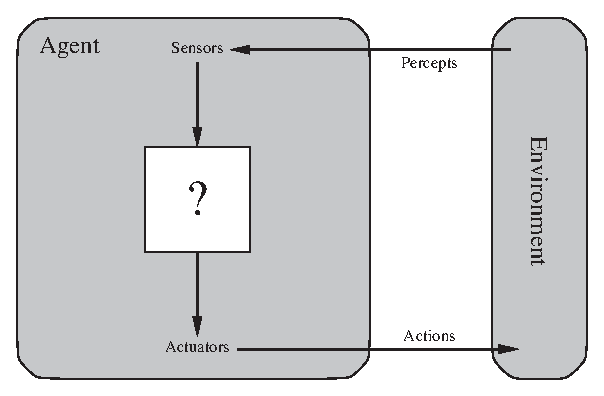
\includegraphics{Chapters/BackgroundKnowledgeAndRelatedWork/Figs/Vector/agent-environment.eps}
    \caption{Agent-Environment Interaction (Russell and Norvig)\cite[p.~35]{AIAMA}}
    \label{fig:agent_env_interaction}
\end{figure}
The box containing the question mark represents the agent's internal decision-making process, which generally speaking involves choosing an action, given the complete history of everything that the agent has perceived. The mapping from percept sequences to actions is described as the agent function. The agent function is an abstract notion; at a lower level an agent program implements the agent function, running on some physical system. A key concept in developing an agent program is rationality: "\textit{for each possible percept sequence, a rational agent should select an action that is expected to maximize its performance measure, given the evidence provided by the percept sequence and whatever built-in knowledge the agent has}"\cite[p.~37]{AIAMA}. This thesis is concerned with designing a system of agents that should exhibit rational behaviour.\newline
 

Russell and Norvig group agents into four common classes based on the design of the agent function\cite[p.~47]{AIAMA}: 
\begin{enumerate}
    \item \textbf{Simple reflex agents}: These agents select actions to take by ignoring the percept history to date, with the exception of the most recent percept.
    \item \textbf{Model-based reflex agents}: These agents have an internal state that depends on the percept history and is updated using new percepts. Updates occur using a model of the world.
    \item \textbf{Goal-based agents}: These agents are an extension to model-based reflex agents. They have some information about whether they have reached a "goal" state, which is desirable. The agent can choose actions to take based on the model. \note{Define what a goal state is.}
    \item \textbf{Utility-based agents}: A utility function is used as an internal performance measure in order to select actions. This allows an agent to pick among actions that may not immediately lead to a goal state.
\end{enumerate}
Recent work in the field of AI has strongly focused on learning agent architectures, which is a superset of all of the above agents. The key difference between the agent types listed above and a learning agent is that a learning agent has the ability to improve its performance through time independently. Its decision making process is not necessarily static and can change beyond its initial programming. An explanation of the architecture of a learning agent can be found in Russell and Norvig \cite[p.~55]{AIAMA}. Implementing each of these different types of agents requires varying degrees of effort. Depending on the problem, different architectures may be more or less suited, which suggests that fully understanding the problem that is attempted to be solved is of fundamental importance when designing an agent.

\subsection{Multi-Agent Systems}
Analogous to the definition of an agent, there is no universally agreed-upon definition of a \emph{Multi-Agent System} (MAS). A definition is provided in a field review paper by Stone and Veloso: "\textit{Multiagent Systems (MAS) is the subfield of AI that aims to provide both principles for construction of  complex  systems  involving  multiple  agents  and  mechanisms  for  coordination  of  independent  agents’ behaviors}" \cite{Stone2000MultiagentPerspective}. While the design of individual agents tends to focus on maximising a performance measure, the design of a multi-agent system is rather more multi-faceted. Weiss \cite{MAS:AModernApproachToDAI} notes that it is almost always oriented towards answering the question of "\textit{when and how to interact with whom}". Multi-agent systems have been proposed as a solution to many problems that modern AI attempts to tackle for some of the following reasons, which are outlined in more depth in \cite{Stone2000MultiagentPerspective}: 
\begin{itemize}
    \item Some problems by definition can be described as a multi-agent system. An example is an organization that may want to model it's internal affairs with a single system. The different departments have their own sub-systems that have differing priorities and capabilities; their interactions naturally can be thought of as interactions between independent agents, in accordance with the definition provided at the start of this section.
    \item The accomplishment of a task can be expedited significantly by using multiple agents. Multi-agents systems are part of the field of Distributed Artificial Intelligence (DAI) and so problem domains that decompose into several independent tasks that can be handled by separate agents can benefit from their use. The problem of efficient task allocation in multi-agent systems has been well-studied in the literature\cite{Gerkey2004ASystems}. 
    \item Robustness is an often-cited benefit of multi-agent systems. Distributed control means that failure of a single agent (mechanical or otherwise) may be tolerated.
    \item Multi-agent systems are often more scalable than single-agent systems. The necessary modularity of multi-agent systems means that adding new agents to the system can often be a solution to a more difficult problem, rather than adding new capabilities to a monolithic system. 
    \item The modularity of multi-agent systems means that the design and programming of them may be simplified. For example, rather than solving a multi-objective problem with a single agent, a single-objective problem may be solved with multiple agents. A result of this is that multiple cheap robots may be used to outperform a single, expensive robot \cite{Grabowski2000HeterogeneousExploration}.
\end{itemize}
\par



\section{Multi-Agent Stochastic Target Localization}
\workinprogress

A problem explored in this thesis is an instance of target detection using a system of aerial robots. A more primitive version of this problem initially gained traction in the literature with the work of Koopman \cite{KoopmanTheoryOfSearchTargetDetection} and has received much attention since. More recent papers have framed the problem in terms of agents and multi-agent system. %Citations needed
A common feature in the problem definition in the literature is that the system of agents are assumed to work in a partially observable environment\cite{Symington2010ProbabilisticUAVs}, \cite{Chung2008Multi-agentFramework}, \cite{WongMulti-vehicleTargets}. Many recent approaches follow the groundwork laid by Elfes\cite{ElfesUsingNavigation}, whereby an "occupancy field" is used to represent the distribution of the target over the cells of a spatial lattice. Elfes describes an Occupancy grid as a "probabilistic tesselated representation of spatial information". This is in contrast to previous approaches that typically used geometric models of the world, which enforced strong domain-specific dependencies. The occupancy field framework 
\par

%Should reference stone as well as koopman

\section{Multi-Agent Coverage Problem}
\input{Chapters/BackgroundKnowledgeAndRelatedWork/MultiAgentCoverageReview.tex}

\section{Simulation Environments}
%Want to introduce the problem to allow for a discussion that makes sense. Ideally will frame a problem so that it suggests that having a high-fidelity simulation environment would be very useful for the project and in general.
\subsection{Key Aspects of Simulation Environments}
According to \citeauthor{Shannon1998INTRODUCTIONSIMULATION} \cite{Shannon1998INTRODUCTIONSIMULATION}, simulation can be defined as \textit{ the process of designing
a model of a real system and conducting experiments with
this model for the purpose of understanding the behavior of
the system and /or evaluating various strategies for the
operation of the system}. Simulations have been used extensively to model complex systems since the invention of the modern computer, gaining traction since the proposal of the Markov Chain Monte Carlo method by Stansislaw Ulam and John Von Neumann in the late 1940s \cite{Robert2011AIncomplete}. Simulations written with software are usually created in order to gain insight into the system's dynamics and to evaluate results of using a method intended for use in the real world. This is usually because proposed methods may be too time-consuming or expensive to test in the real world. Software simulations are being used increasingly for a wide variety of tasks, from planning new roads to alleviate traffic \cite{Pell2017TrendsSimulation} to developing self-driving vehicles \cite{Dosovitskiy2017CARLA:Simulator}. 

Designing simulations allows the developer of an agent-based system to abstract away details of the real-world conditions that the agents will act in and focus on the salient aspects that the agents are concerned with, in order to prototype, train, test analyse and validate. General advantages of simulations are listed in  \cite{Shannon1998INTRODUCTIONSIMULATION}, with the most notable being:
\begin{itemize}
    \item \textit{It can be used to explore operating procedures, decision rules, organizational structures, etc. without disrupting the ongoing operations.}
    \item \textit{Simulation allows us to control time. Thus we can operate the system for several months or years of experience in a matter of seconds allowing us to quickly look at long time horizons or we can slow down phenomena for study.}
    \item \textit{It allows us to gain insights into how a modeled system actually works and understanding of which variables are most important to performance.}
    \item \textit{Simulation's great strength is its ability to let us experiment with new and unfamiliar situations and to answer "what if" questions.}
\end{itemize}


\note{Following paragraph doesn't really belong here but does help tie everything together}

 In relation to designing intelligent agents, often the trade-off between exploration and exploitation is referenced. Exploration or "information gathering" \cite{AIAMA} can be considered as the agent posing a "what if" question in order to learn the consequences of performing action, and exploitation can be considered as an agent using gathered or previous knowledge to choose actions to take that maximize its performance measure, as outlined in section \ref{AgencySubsection}. As stated above, simulation environments are highly suited to answering "what if" questions, which has motivated the use of using simulations to design systems of autonomous agents in the literature, for example the simulation environment used in the 
\href{https://multiagentcontest.org/}{Multi-Agent Programming Contest.}\footnote{\href {https://multiagentcontest.org/}{https://multiagentcontest.org/}}



\subsection{Using Game Engines to Design and Generate Simulation Environments}\label{GameEngineReview}
Since computer games are effectively simulations, the technologies used to create them have also been used to create simulations for a more serious purpose, often referred to in the literature as \textit{serious games}. Serious games usually refer to games that have been specifically designed to provide training to professionals working in an industry where extensive training is necessary but difficult, expensive or dangerous to provide. An overview and taxonomy of serious games is provided by \citeauthor{Laamarti2014AnGames} \cite{Laamarti2014AnGames}. More recently, games have been used to train learning agents, described in \ref{AgencySubsection}. This is because game engines have reached a level of maturity that can provide high-fidelity percepts to agents in order to replicate the true environment they would like to perform in. Initially, manufacturing created a demand for simulation technology, since taking a manufacturing plant offline in order to integrate new robotics technology could cost a company a significant amount of money. Simulink, developed by Matlab, was initially a popular tool to develop models of dynamical systems, but it's limitations include ...

Since highly influential papers related to 


Modern-day games are commonly written using a \textit{game engine}, rather than being designed from the bottom up as a singular entity. There is no strict definition for what constitutes a game engine, but the term usually describes a software development environment which typically provides functionality including some kind of rendering engine for 3D graphics, a physics engine that deals with phenomena such as collision, a sound engine, networking abilities, memory management, threading, cinematics and animation. This functionality is necessary in most modern games and has been developed to economise the process of game development.\par



\subsection{AirSim Simulator}



Games engines have developed
In the context of ROCSAFE and 



We have identified the following aspects of the real-world scenario we hope to address as causing issues in developing our system:
This motivates the development of a high-fidelity simulation to circumvent these limitations.



Simulations are typically of high value when data required to design system:
\begin{itemize}
    \item Costs a lot of money to generate.
    \item Is dangerous to generate.
    \item Is time consuming/laborious to generate.
    \item The system has a well-known stochastic element which makes generating a sufficiently large sample size difficult.
\end{itemize}
The domain which motivated the development of the technologies proposed in this thesis satisfies all of the above requirements, which naturally motivates the design of a simulation environment. \par

 Key properties of a simulation 

%Intelligent agents are frequently designed to solve problems which usually would be on or more of: labour intensive, monotonous, repetitive or time consuming. In order to accomplish these tasks, agents may need to use data from 

Simulation environments are used to solve a number of different problems when using intelligent agents.

A consequence of this is that any systems that are developed to provide support can be difficult to evaluate and validate. To address this, we developed a high-fidelity simulated environment as part of the research involved in this thesis, which preserves the critical aspects of CBRNe incidents without presenting any risk of exposure to the dangerous elements of such scenes in the real world. The following published works related to the development of the simulation environment are discussed in this chapter: \citet{Smyth2018AInvestigation}, \citet{Smyth2018UsingDrones}.\par


Virtual environments designed using games engines have previously been used to gather data to train models for a range of applications \cite{1608.02192}\cite{uav_benchmark_simulator} and software packages have been written that can generate photo realistic images from games engines\cite{1609.01326}. There have also been attempts made to develop models of physical systems that simulate potentially dangerous environments \cite{4625089}. To the best of our knowledge, there are no prior applications using games engines to model critical incidents for the purpose of developing analytical tools in a virtual setting that will then transfer to real-world deployment.

